\section{Merge Sort} \label{cap:2:section:msort}

\subsection{Introdução}

O \textit{Merge} Sort é um algoritmo de ordenação bastante eficiente, seu funcionamento é baseado
na estratégia de ordenação de dividir para conquistar. Basicamente, o processo de ordenação consiste
em separar de forma recursiva o vetor, até que contenha 1 elemento e então, realiza o procedimento
\textit{merge}, que consiste produzir um novo vetor ordenado dos elementos de mesma profundidade
topológica.

\subsection{Implementação}

Para o algoritmo de ordenação por mesclagem, o pseudo-código utilizado para desenvolver o
algoritmo pode ser observado em \ref{mergeSortP}.

\begin{pseudocode}[caption={Algoritmo de ordenação por mesclagem}, label={mergeSortP}]
MERGE-SORT(A, l, r)
if l < r then
    m $\gets$ l + (r - l) / 2

    MERGE-SORT(A, l, m)
    MERGE-SORT(A, m + 1, r)

    MERGE(A, l, m, r)
\end{pseudocode}

Esse pseudo-código foi implementado na linguagem de programação C 
e pode ser observado no código seguinte:

\begin{lstlisting}[style=CStyle]
void merge(int * v, int l, int m, int r) 
{ 
    int i, j, k; 
    int n1 = m - l + 1; 
    int n2 = r - m; 

    int L[n1], R[n2]; 
    
    for (i = 0; i < n1; i++) 
        L[i] = v[l + i]; 
    for (j = 0; j < n2; j++) 
        R[j] = v[m + 1 + j]; 
    
    i = 0; 
    
    j = 0; 
    
    k = l; 
    while (i < n1 && j < n2) { 
        if (L[i] <= R[j]) { 
            v[k] = L[i]; 
            i++; 
        } 
        else { 
            v[k] = R[j]; 
            j++; 
        } 
        k++; 
    } 
    
    while (i < n1) { 
        v[k] = L[i]; 
        i++; 
        k++; 
    } 
    
    while (j < n2) { 
        v[k] = R[j]; 
        j++; 
        k++; 
    } 
} 

void mSort(int * v, int l, int r) 
{ 
    if (l < r) { 
        int m = l + (r - l) / 2; 
  
        mSort(v, l, m); 
        mSort(v, m + 1, r); 
  
        merge(v, l, m, r); 
    } 
} 
\end{lstlisting}

\subsection{Análise do algoritmo e notação assintótica}

Para que seja determinada a razão de crescimento do algoritmo de ordenação por mesclagem, é necessário
perceber os tempos de execução de cada linha do pseudo-código \ref{mergeSortP}.
Nesse caso, pode-se ter como base a equação \ref{cap:2:eq:mergeSort:1}.

\begin{equation} \label{cap:2:eq:mergeSort:1}
    T(n) = \sum_{i=1}^{\log n}(C_2 + C_3 + T(MERGE))
\end{equation}

Sabendo que, o tempo de execução $T(MERGE) = O(n)$, podemos assumir a relação entre a equação 
\ref{cap:2:eq:mergeSort:1} com a equação \ref{cap:2:eq:mergeSort:2}.

\begin{equation} \label{cap:2:eq:mergeSort:2}
    T(n) = a \times \log n + c\  para\  a = (C_2 + C_3 + T(MERGE))
\end{equation}

Com isso, pode-se determinar as seguintes notações assintóticas para o algoritmo de ordenação por mesclagem:

\begin{align*} \label{cap:2:eq:mergeSort:3}
    O(n) &= n \times \log n \\ 
    \Omega(n) &= n \times \log n \\
    \Theta(n) &= n \times \log n
\end{align*}

\subsection{Comparação teórica-prática}

Para melhor compreensão do tempo de execução do algoritmo de ordenação por mesclagem, pode-se observar o gráfico 
\ref{cap:2:graph:mergeSort} que apresentam o tempo de execução para o algoritmo de ordenação por mesclagem
para 8192 casos diferentes com o número de entradas $n$ variando de 1 a 1048576.

\begin{figure}[h]
    \centering
    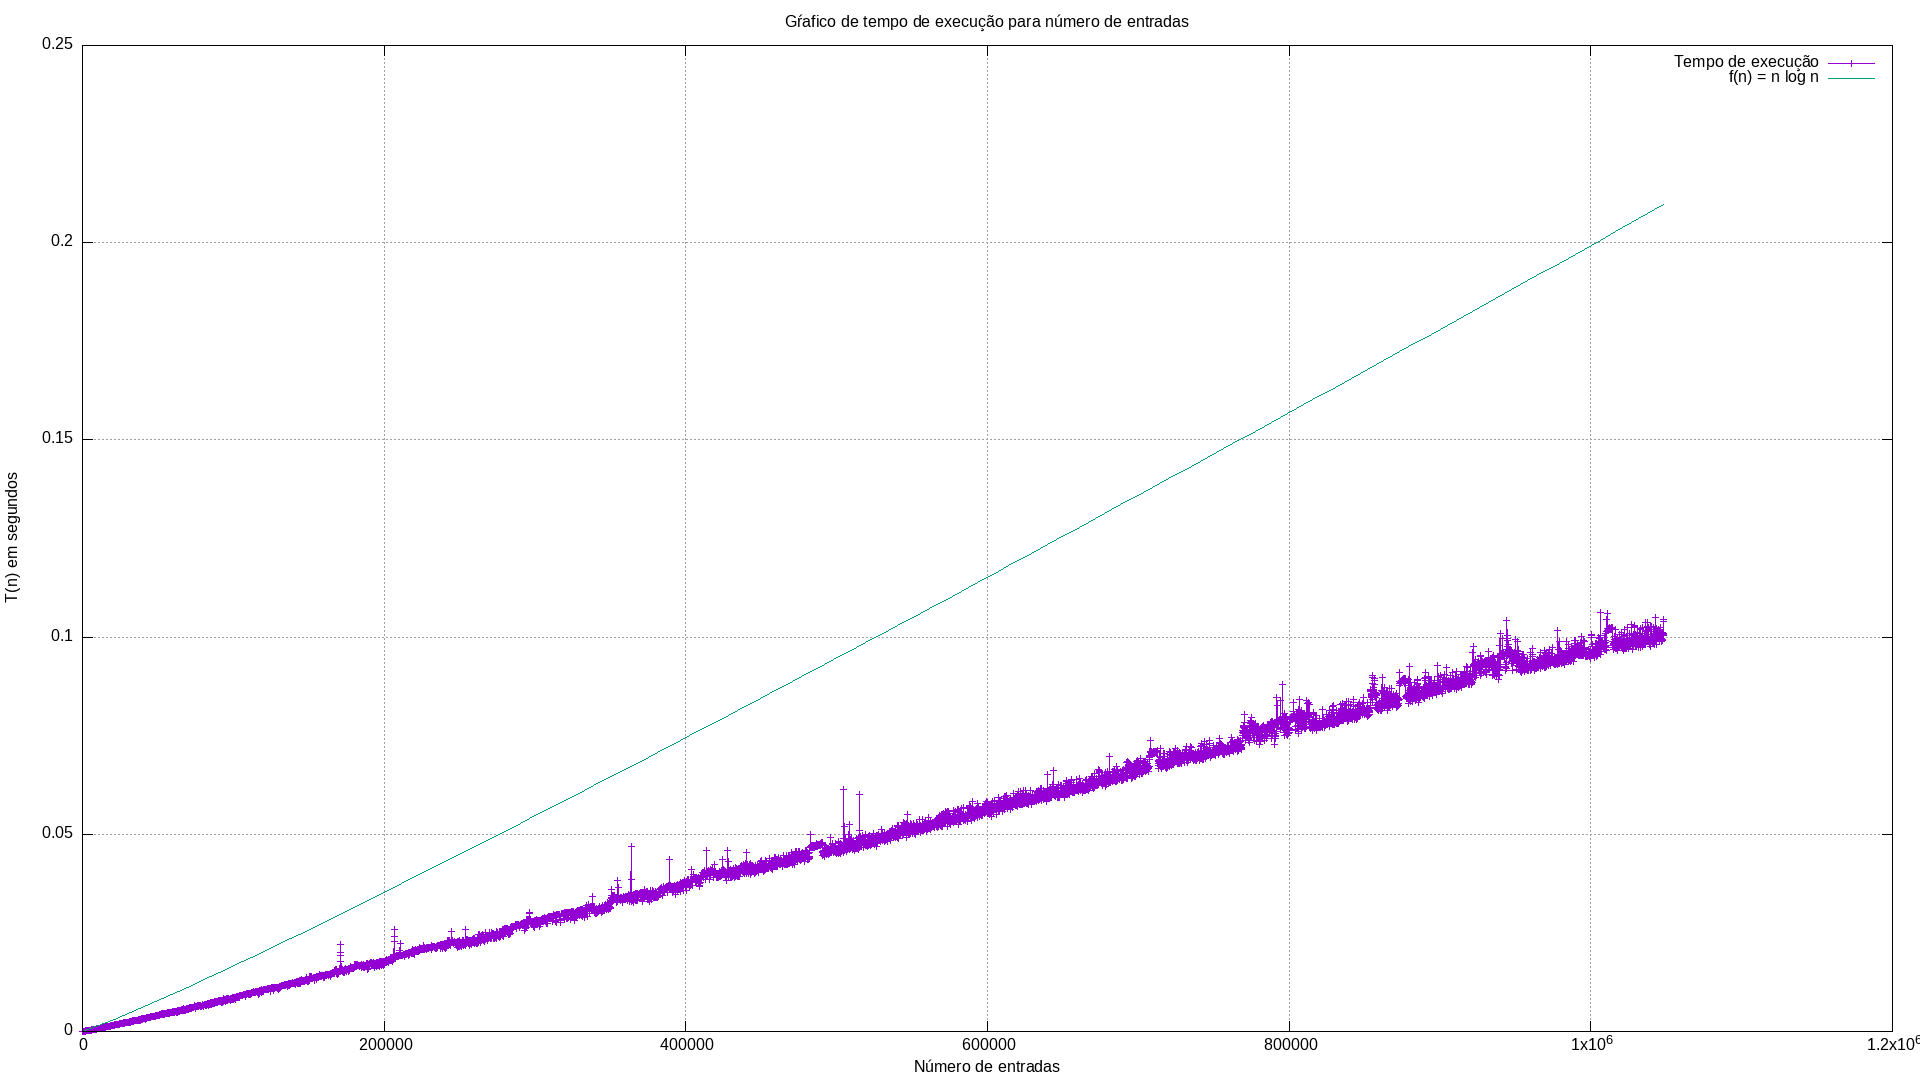
\includegraphics[width=\textwidth]{image/graphics/mergeSort.png}
    \caption{Gráfico com tempo de execução do algoritmo de ordenação por mesclagem}
    \label{cap:2:graph:mergeSort}
\end{figure}

No gráfico \ref{cap:2:graph:mergeSort}, é possível perceber que o tempo de execução do algoritmo se aproxima
da função $f(n)$ que é uma função $n \times \log n$ para $n$ com uma redução de escala para melhor percepção e comparação. Então,
utilizando como base o gráfico \ref{cap:2:graph:mergeSort}, pode-se confirmar que a ordem de crescimento determinada é
precisa.

\subsection{Discussão sobre tempo de execução e uso de memória}

Sobre seu tempo de execução, o algoritmo de ordenação por mesclagem é eficiente para
vetores com muitas entradas. Sobre seu uso de memória, é na ordem de $S(n) = n$ porque utiliza vetores auxiliares
que crescem de forma linear com $n$.

